\documentclass[whitelogo]{tudelft-report}
\usepackage{natbib}
\usepackage{changes}
\usepackage[natbibapa]{apacite}
\usepackage{todonotes}
\begin{document}

%% Use Roman numerals for the page numbers of the title pages and table of
%% contents.
\frontmatter

%% Uncomment following 19 lines for a cover with a picture on the lower half only
%\title[tudelft-white]{Title}
%\subtitle[tudelft-cyan]{Optional subtitle}
%\author[tudelft-white]{J.\ Random Author}
%\affiliation{Technische Universiteit Delft}
%\coverimage{cover.jpg}
%\titleoffsetx{10cm}
%\titleoffsety{10cm}
%\afiloffsetx{1cm}
%\afiloffsety{18cm}
%\covertext[tudelft-white]{
%    \textbf{Cover Text} \\
%    possibly \\
%    spanning 
%    multiple 
%    lines
%    \vfill
%    ISBN 000-00-0000-000-0
%}
%\makecover

%% Uncomment following 16 lines for a cover with a picture on the lower half only
\title[tudelft-white]{A Robot Economy for Music Without Any Middleman}
% \subtitle[tudelft-black]{Optional subtitle}
\author[tudelft-white]{Tim Wissel}
\affiliation{Technische Universiteit Delft}
% \coverimage{tank.jpg}
% \covertext[tudelft-white]{
%     \textbf{Cover Text} \\
%     possibly \\
%     spanning 
%     multiple 
%     lines
%     \vfill
%     ISBN 000-00-0000-000-0
% }
\setpagecolor{tudelft-cyan}
\makecover[split]


%% Include an optional title page.
\begin{titlepage}


\begin{center}

%% Insert the TU Delft logo at the bottom of the page.

%% Print the title in cyan.
{\makeatletter
\largetitlestyle\fontsize{32}{32}\selectfont\@title
%\largetitlestyle\color{tudelft-cyan}\Huge\@title
\makeatother}

%% Print the optional subtitle in black.
{\makeatletter
\ifx\@subtitle\undefined\else
    \bigskip
   {\tudsffamily\fontsize{22}{32}\selectfont\@subtitle}    
    %\titlefont\titleshape\LARGE\@subtitle
\fi
\makeatother}

\bigskip
\bigskip

by
%door

\bigskip
\bigskip

%% Print the name of the author.
{\makeatletter
%\largetitlefont\Large\bfseries\@author
\largetitlestyle\fontsize{26}{26}\selectfont\@author
\makeatother}

\bigskip
\bigskip

to obtain the degree of Master of Science
%ter verkrijging van de graad van Master of Science

at the Delft University of Technology,
%aan de Technische Universiteit Delft,

to be defended publicly on XXX at XXX.
%in het openbaar de verdedigen op dinsdag 1 januari om 10:00 uur.

\vfill

\begin{tabular}{lll}
    Student number: & 4460251 \\
    Project duration: & \multicolumn{2}{l}{March 6, 2020 -- XXX} \\
    Thesis committee: & Dr.\ ir.\ J.\ Pouwelse, & TU Delft, supervisor \\
        % & Dr.\ E.\ L.\ Brown, & TU Delft \\
        % & Ir.\ A.\ Aaronson, & Acme Corporation
\end{tabular}
%% Only include the following lines if confidentiality is applicable.

\bigskip
\bigskip
An electronic version of this thesis is available at \url{http://repository.tudelft.nl/}.
%\\[1cm]

%\centering{
\includegraphics{cover/logo_black}}


\end{center}

\begin{tikzpicture}[remember picture, overlay]
    \node at (current page.south)[anchor=south,inner sep=0pt]{
        
\includegraphics{cover/logo_black}
    };
\end{tikzpicture}

\end{titlepage}



\chapter*{Preface}
\setheader{Preface}

Preface\ldots

\begin{flushright}
{\makeatletter\itshape
    \@author \\
    Delft, March 2020
\makeatother}
\end{flushright}



\tableofcontents

%% Use Arabic numerals for the page numbers of the chapters.
\mainmatter

\chapter{Introduction}
\label{introduction}
Music streaming services have an immense amount of power in the music industry. The biggest streaming services dictate the rules which artists have to play by. The top 5 streaming services and the top 3 labels dominate the market. Artists have a hard time to make a living because the streaming companies take large revenue cuts. The centralization of power on Internet platforms cause unfairness in multiple industries, of which the music industry is particularly affected. This thesis aims to distribute the power from centralized streaming platforms to listeners and artists.

The music streaming industry is completely digital\; from recording and publishing to listening and digital rights management. We investigate the feasibility of fully replacing this digital value chain by software. 

\todo[inline]{Insert clear Robot Economy definition, Insert contributions and goals of this thesis}
% Een problem begin zoals dit:
% The robot economy is already here.Instead, we are still suffering big stagnation; income polarisation is rapidly increasing, wages have been falling, and the rate of technological progress is slowing down. In addition, the latest wave of digital innovation has resulted in excessive returns to capital, with a massive amount of cash going to the balance sheets of big tech companies, while very little is invested in welfare, social infrastructures, education, health and clean energy. This situation is exacerbated by the apparent inability of governments to tax profits made by hi-tech and financial giants, as seen, for instance, in the very generous tax settlement between Google and the government. 
% https://www.opendemocracy.net/en/can-europe-make-it/robot-economy-full-automation-work-future/

\section{Monopolization on the Internet}
The Internet is moving from a network of people to a sparse selection of platforms over which nearly all commerce is regulated. A few Big Tech corporations are gaining increasing power in the the surface on which market exchange takes place. The consumer choice is diminishing due to the power of oligarchs and monopolies. As explained by \citep{stiglitz2019market}, there is a fundamental problem: the growing ``concentration of market power, which allows dominant firms to exploit their customers and squeeze their employees, whose own bargaining power and legal protections are being weakened'', while ``[...] CEOs and executives are extracting higher pay for themselves''.

\section{Centralization of power in the music industry}
An industry with great consequences of this trend is the music industry. In the last 20 years there has been a remarkably fast shift from the exchange of CDs in various stores to music streaming on the Internet. Music platforms and labels use their economic muscle to push down artist salaries. They take large cuts of revenue from the user subscription money.

Firstly, corporations with power squeeze the music production side by taking large cuts of revenue from the user subscription money. As a result, the artists receive a low compensation. Especially independent artists have a hard time making a living. The distributors Spotify, iTunes and Google Play take on a 25\% to 40\% revenue cut.

Secondly, Big Tech has curatorial power to decide what is shown in the catalog of their application. The music catalog may seem endless, but in reality it is controlled by the Big Tech corporation and dictated by the interests of major labels. The inner workings of recommendation algorithms and playlists are in the hands of a few labels and streaming services.

Finally, the streaming companies can sensor tracks. The freedom of artist expression is then decided by undemocratic judgments. Big Tech has the power to decide the future of an artist.

\section{Proposed solution: MusicDAO}
This thesis proposes an alternative technology from Big Tech streaming services. We design and implement a decentralized system which attempts to replace the full value chain in music streaming industry, from the subscription money to the artist, by removing all intermediaries and giving power back to the artists and listeners. Listeners can stream music without being dependent on a single provider and can give money directly to artists. Artists receive 100\% of this donation and subscription money.

In essence, the solution is a decentralized autonomous organization (DAO) which is formed by listeners and artists. A DAO is defined by \cite{buterin2014dao} as an ``entity that lives on the internet and exists autonomously, but also heavily relies on hiring individuals to perform certain tasks that the automaton itself cannot do'' (see \ref{fig:dao-quadrants}). In this thesis we present the design and implementation of our mobile android app MusicDAO: a music streaming service for the common good. Users of this app form a phone-to-phone zero-server network over which they publish music, download music and transfer money. This proof-of-principle of a DAO shows a fair and transparent music streaming service in which no external servers, third parties or intermediaries are necessary. Any person can join the network, publish music and get paid for it. 

MusicDAO supports the following functionalities:
\begin{itemize}
    \item Defining and publishing music content with metadata;
    \item Streaming music over BitTorrent;
    \item Caching and streaming optimization algorithms;
    \item Browsing playlists;
    \item Remote keyword search;
    \item Peer-to-peer donations to artists using Bitcoin.
\end{itemize}

\subsection{Experimentation and evaluation}
In a real-world experiment with Android phones, we tested the feasibility of such a phone-to-phone serverless system. We ran MusicDAO on at least X android devices, and registered the latency of retrieving music metadata, and transaction speeds of transferring money and audio files. 

% Music artists have a hard time making a living. The oligarchical power of music streaming services and labels squeeze  the  production  size  of  the  music  industry
% Stolen from Resonate.is:
% The music industry is dysfunctional. Power has become consolidated in the hands of a small number of technology companies and dominant major labels.
\begin{figure}
	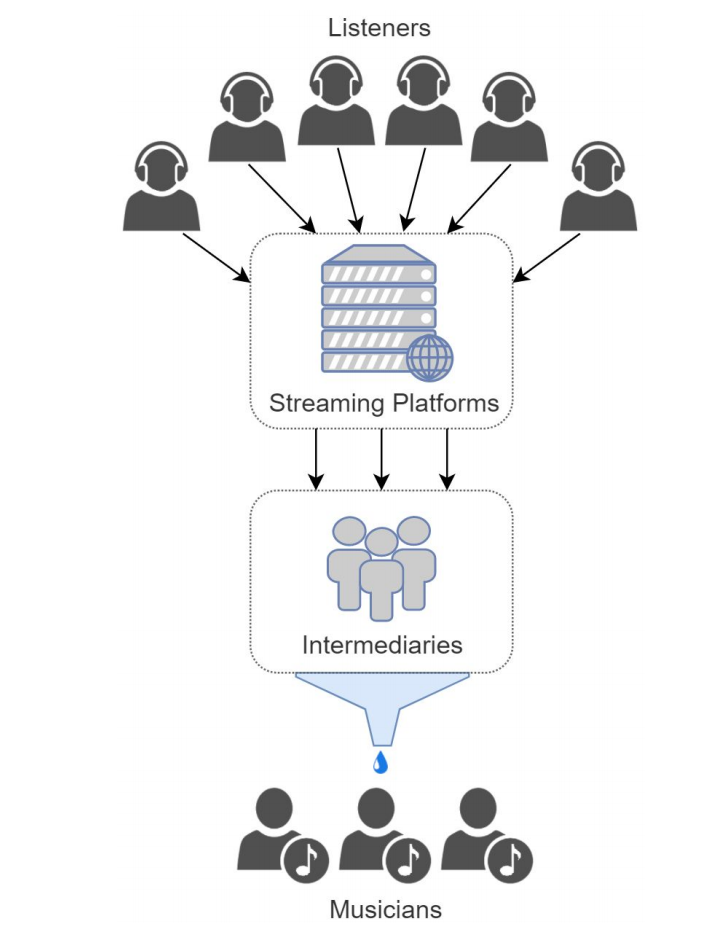
\includegraphics[width=0.4\textwidth]{introduction/problem-image.png}
	\caption{Artist compensation inconsistency}
\end{figure}

% Section X describes the design of the system, section Y its implementation and Z its testing results.
% Most important: How can artists distribute and sell their work in a digital economy beholden to ruthlessly commercial and centralized interests?
% https://thebaffler.com/salvos/the-problem-with-muzak-pelly

% From Audius Whitepapter:
% We see a number of specific challenges faced by creatorsand listeners today:1.  There is little to no transparency around the originsof creator payouts (e.g.  number of plays, location,original gross payment before fees)2.  Incomplete  rights  ownership  data  often  preventscontent  creators  from  getting  paid;  instead,  earn-ings accumulate in digital service providers (DSPs)and rights societies3.  There are layers of middlemen and significant timedelay involved in payments to creators4.  Publishing rights are complicated and opaque, withno incentives for the industry to make rights datapublic and accurate5.  Remixes,  covers,  and  other  derivative  content  arelargely censored due to rights management issues6.  Licensing issues prevent DSPs and content from be-ing accessible worldwide

\chapter{\label{chap:related-work}Problem description}
% Centralization of data, with the incentive of making money, naturally leads to a centralization of power. 
The most widely used music streaming services, with the largest music catalogs, run centralized, proprietary and cosed-source software. The companies owning these services have a large amount of power in the music streaming industry because of their scale. The top 5 streaming services have a combined market share of 81\%, so this can be regarded as an oligarchy. Because of their power, they can ask high commission fees or lock artists to one platform. As a result, artists receive low compensation. Furthermore, in closed-source software, the processing and storing of user data is nontransparent. The recommendation and playlist generation algorithms are also a black box for the user. As companies make money from selling data to third parties, their data-gathering methods are expected to become more disruptive for user privacy. At the time of writing, there exists no alternative decentralized and transparent music streaming system without intermediaries.

\textit{How can we design and implement a music streaming service that distributes the power from one authority to its users?}% \subsection{Ownership} ? It may be true that when you purchase a record on iTunes or favourite something on Spotify, you do not legally own a copy of it but only an access to it via their proprietary closed source platform.
\subsection{Intermediaries take a large share}
Artists publishing their content on Big Tech music platforms such as Google Music, Spotify and iTunes receive low compensation, because the intermediaries take a large share. According to Midia Research, the top 5 most popular music streaming services control 81\% market share\cite{midiamarketshare2020}, which can be regarded as a  Specifically, these companies take on average a 25 percent cut for signed records, and a 40 percent cut for unsigned records\footnote{\url{https://www.theguardian.com/technology/2015/apr/03/how-much-musicians-make-spotify-itunes-youtube}}. 
% In addition, these platforms use a "pro rata" model, meaning that the artists are paid per amount of plays per month. This model makes it more difficult for small, independent artists to make a living \todo{add sources}. 
% Content creators on the Internet receive a low compensation for publishing their content on monopolize
% Expand upon: small independent artists. Smaller artists get low revenue, due to the "pro rata" model applied by e.g. Spotify. A user-centric model should be more fair.
\subsection{Monopsony power}
% \section{Centralization of power}
% Centralization of data, with the incentive of making money, naturally leads to a centralization of power
Monopsony power means that a dominant buyer has the power to push prices down with suppliers. In the context of music, this means that artists have little choice over which platform to publish their music on, because of the dominance of one platform. A few major players in the music industry together form an oligopolistic market. Monopsony power in this area can lead to squeezing the producer side. An example of monopsony power is an event that happened in 2014, between Amazon and Hachette. Amazon, having a large market share on e-books, used its commercial muscle to demand a larger cut of the price of Hachette books it sells. This included for all Hachette books ``preventing customers from being able to pre-order titles, reducing the discounts it offered on books and delaying shipment''\cite{theguardian2014amazon}. Along the same lines, Spotify can use its commercial muscle to demand low pays to artists. If some artists are not willing to cooperate, Spotify can deliberately remove their content from its recommendations, such as from the Discover Weekly playlists. Spotify claims that over 10 billion times a month, listeners across both Spotify and Spotify Premium stream a new artist they had never heard before. So their recommendation system is highly influential for its users.
\subsection{Transparency of user data processing}
Big Tech companies obtain personal usage data to be able to improve their service, but also to to sell the data to third parties for a profit. In this process, users must heavily trust the company running the service to handle their data exactly as stated in their privacy policy. In the scope of music streaming services, user data such as browsing activity, and friends and sharing activity is obtained. For instance, Spotify saves personal usage data such as ``search queries [...], streaming history, playlists you create, your library, your browsing history, and your interactions with the Spotify Service, content, other Spotify users.'' and shares this data with advertising parties, stated in their privacy policy\footnote{\url{https://www.spotify.com/us/legal/privacy-policy}}. Google Music ``shares, processes, and maintains information about your usage, access, and playback of Your Music [...], playback activity related to items you preview and buy in the Google Music Store ("Store Usage"); and about the songs you share and listen to in connection with Google Music Social Recommendations [...]'' as described in their privacy policy\footnote{\url{https://music.google.com/about/privacy.html?em_x=22}}. 

Following the lack of privacy comes issues with what companies do with all the user data they gather. Widely known is the use of this data for targeted advertising\cite{jessup2012big} and for selling as a profit\cite{yap2011user}. A risk in this process is that the third parties may use this private information for malicious purposes\cite{yap2011user}. From the perspective of the user, there is no transparency for whether this happens. According to \cite{narayanan2008robust}, privacy may be breached even when a service is willing to protect a user's privacy, because state-of-the-art de-anonymization methods do not fully make users anonymous, depending on the features stored in the database. Centralized software services are subject to a single point-of-failure. In this context this involves the risk of security breaches: if a malicious party gains access to its database, all of the records can be leaked at once which can lead to a large-scale privacy breach. Furthermore, \cite{dworkdifferential} shows that such an event can leak personal data of users who are not part of the original database.
% Integrations with IoT devices and sensors are in development which may lead to more invasion of privacy in the future.
% \subsection{Control of data}
% The GDPR contains the right for individuals to have their data erased from any platform. However, a user taking this action cannot be certain of this happening on request, as access to the companies' database is not available from the outside. Furthermore, the company implements disclosure preferences in the way they see fit, which may not be fine-grained. 
\subsection{Content censoring}
The company running the software is free in how and which content to censor. In addition, their content censoring policy may be changed at any time. Recent examples exist such as the disappearance of Li Zhi\footnote{\url{https://www.independent.co.uk/news/world/asia/tiananmen-square-china-li-zhi-singer-disappears-anniversary-protests-a8940641.html}}, who published songs about democracy and social issues in China. All of China's main streaming sites removed his songs. In 2019, Apple Music removed content from their platform by singer Jacky Cheung, who referenced the tragedies of Tiananmen Square in his songs.
\subsection{Recommendation of content}
The Big Tech music companies recommend content that best fits their business model, which may be contrary to what fits the user best. The companies can promote or dis-promote content by their choosing. For example, on Spotify, brands are able to sponsor playlists. ``A car company might sponsor a popular driving playlist on Spotify''\cite{prey2018nothing}. As the companies run closed-source software, the recommendation engine they use are a black box to the user. They are not obliged to explain the algorithms used for this. Small, independent artists may suffer from labels that invest large amounts of money to have their content promoted.
\subsection{Security and fault tolerance}
As the service and software are proprietary, and the running code is closed-source, there are security risks. Specifically, the cryptography and security mechanisms used internally can not be inspected by people outside of the company. \todo[inline]{expand}
% \subsection{Server costs} ? (This is not really a problem from the perspective of user and/or artist? Unless there are sources that say otherwise)
\subsection{Resiliency}
At any point in time, the company running proprietary software can change, add or remove features. Its users do not necessarily have a vote in this. When a software service is sold to a different owner, the new owner can completely change direction for the service, which makes the service prone to large, possibly unwanted changes. Moreover the company can decide to take down the service in its entirety. For example: In 2017, Pandora discontinued running its service in New Zealand and Australia\footnote{\url{https://www.businessinsider.nl/pandora-shutting-down-services-australia-new-zealand-2017-7?international=true&r=US}}. In this case, users can lose all their data stored on the service.
% All the evidence suggests a description of an oligopolistic market - a few large providers with high market share, interdependence based upon pricing (chance for a kinked demand curve to be drawn, if your awarding body still uses that model!) and only slightly differentiated products.
\subsection{Platform locking}
As an example from YouTube, a company can disallow content creators to publish their work on other platforms, resulting creators to be locked to one platform. \todo[inline]{Find sources of this happening}  
% \subsection{Oligopoly formation}
% Also, a natural consequence: (Unnecessary high) pricing of content. When a monopoly on music content is formed, the Big Tech companies can together decide to up the price 'whenever they feel like it'.
% \subsection{Copyright orthodoxy} ?
% % https://search.proquest.com/openview/2ea25b1bed66750c91cdbc6ea2a5093a/1
% \subsection{Low level of innovation} ?

% \todo[inline]{Software quality measurements: functionality, scalability, maintainability, portability, and, ingeneral, enhancing the usability of the software. See \cite{raghunathan2005open}}

% From Audius Whitepapter:
% We see a number of specific challenges faced by creatorsand listeners today:1.  There is little to no transparency around the originsof creator payouts (e.g.  number of plays, location,original gross payment before fees)2.  Incomplete  rights  ownership  data  often  preventscontent  creators  from  getting  paid;  instead,  earn-ings accumulate in digital service providers (DSPs)and rights societies3.  There are layers of middlemen and significant timedelay involved in payments to creators4.  Publishing rights are complicated and opaque, withno incentives for the industry to make rights datapublic and accurate5.  Remixes,  covers,  and  other  derivative  content  arelargely censored due to rights management issues6.  Licensing issues prevent DSPs and content from be-ing accessible worldwide


% Spotify’s front page “Browse” screen presents a classic illusion of choice, a stream of genre and mood playlists, charts, new releases, and now podcasts and video. It all appears limitless, a function of the platform’s infinite supply, but in reality it is tightly controlled by Spotify’s staff and dictated by the interests of major labels, brands, and other cash-rich businesses who have gamed the system. https://thebaffler.com/salvos/the-problem-with-muzak-pelly
% “The more vanilla the release, the better it works for Spotify. If it’s challenging music? Nah,” 
% We should call this what it is: the automation of selling out.
% “The difference now is that, if you don’t bow down to Spotify, you might as well tell whoever runs the guillotine that’s above your neck to just let her rip,” Saunier says, as the band sits in their van, on tour, en route from Grand Rapids to Detroit. “These streaming services are literally the only option for a music career nowadays.”
\chapter{\label{chap:state-of-the-art}State of the Art}
In this chapter we describe existing algorithms, protocols and applications in computer science, which try to solve, or give an alternative for, the centralized power in Big Tech, and more specifically in digital audio streaming. We inspect full solutions in the form of distributed applications, and techniques which solve subproblems, such as decentralized file sharing protocols.
\section{Decentralized music distribution technologies}
Multiple decentralized audio distribution and streaming applications exist. Examples are Audius~\citep{audius2018}, Musicoin~\footnote{\url{http://musicoin.org/}} and Opus Audio~\citep{jia2016opus}.

\subsection{Audius}
Audius~\citep{audius2018} presents a decentralized protocol for audio content, which aims to improve payouts to artists and its transparency. It contains a token economy with a transparent payout system for the artists, and a user-operated, distributed network for metadata and content. In addition, it has a governance system like a DAO, in which users can decide on changes to the protocol by democratic voting. Its protocol is established around the ideology of disintermediation: ``Intermediaries  should  be  removed  when  possible; when necessary, they should be algorithmic, transparent, and verifiably accurate''~\citep{audius2018}. It uses IPFS~\citep{benet2014ipfs} for storage of audio content, meaning it relies on voluntarily-hosted high-performant servers.

\subsection{Opus Audio}
Opus Audio~\citep{jia2016opus} is a decentralized music-sharing platform and proposes a solution for music ownership registration on a blockchain structure. It has a running distributed audio file sharing system using the Inter-Planetary FileSystem designed by \cite{benet2014ipfs} (see \ref{sec:decentralized-content-delivery}). It contains a decentralized and fully automated system for purchasing access to music, which works as follows. Opus stores encrypted audio files on a swarm of connected nodes. The decryption keys and files hashes are stored in a smart contract (see \ref{sec:smart-contracts}). Using cryptocurrency, users spend their funds on these smart contracts, to unlock access to audio files.

\subsection{Musicoin}
Musicoin is a blockchain platform without intermediaries that focuses on income for independent artists. It uses smart contracts and cryptocurrency to show transparency in payments (see \ref{sec:smart-contracts}). This payment structure ensures that each contributor in the network is rewarded, and that artists receive a stable income based on the Universal Basic Income ideology. Aside from their blockchain architecture, they introduce the \$MUSIC cryptocurrency, which they invision as the currency for all economic activity in the music industry. Not all of their architecture is decentralized. They use centralized registration system for artists and listeners. They pay artists using their \$MUSIC currency, of which the value may be highly unstable.s

None of the state-of-the-art decentralized audio streaming technologies show a running, fully decentralized infrastructure with stable income for artists. All of these systems have in common that they save metadata and identifiers of audio files on a blockchain, and save the audio files in an off-chain database using IPFS~\citep{benet2014ipfs}. This makes these solutions reliant on people voluntarily running IPFS content nodes (servers hosting the audio files). In a fully decentralized network, every participant should have the same role, meaning that every node both uploads and downloads content, and it should not be reliant on external servers. Most decentralized systems use their homebrew cryptocurrency to pay artists, instead of a well-established currency or stablecoin. Opus Audio has a development \& marketing fund which take a cut of the music revenue, so not all of the revenue goes directly to artists.

\section{Transparent, automated royalty distribution}
\label{sec:smart-contracts}
The payment to royalties to artists can be described in a transparent and immutable record on a blockchain. In addition, smart contracts can be used to automate payments~\citep{buterin2014next}. Smart contracts are self-executing (no ambiguity) and self-verifying (guaranteeing its statements). In the music industry context, a smart contract can be used for transparent, immutable and automatic payment distribution of royalties. This technique was shown in practice in 2017, when Imogen Heap released the song `Tiny Human'~\citep{heap2017blockchain}. Its distribution of payments to the makers and recorders was written in a smart contract, in the form of a record on the Ethereum blockchain. When a user downloads the corresponding track and makes the payment using cryptocurrency, the forwarding details of the payment are located within the blockchain, and executed as declared on the smart contract.

\section{Decentralized application frameworks}
\label{sec:sote-trustchain}
The TrustChain superapp~\citep{mattskala2020} is a framework for implementing mobile Android decentralized applications. It allows for storing append-only immutable data on TrustChain~\citep{otte2017trustchain} and spreading this data in a phone-to-phone serverless network. It follows the concept of super apps~\citep{kpmg2019superapps}, meaning that it contains many mini-apps which use the same networking interface. The Superapp is an Android app as seen in fig. \ref{fig:trustchain-superapp}. Its mini-apps implement decentralized democratic voting and has bitcoin payment integration, among other features.

\begin{figure}
    \minipage{0.3\textwidth}
        \includegraphics[width=1\linewidth]{related-work/screenshot-superapp.png}
        \caption{Trustchain-Superapp overview}
        \label{fig:trustchain-superapp}
    \endminipage\hfill
    \minipage{0.65\textwidth}
        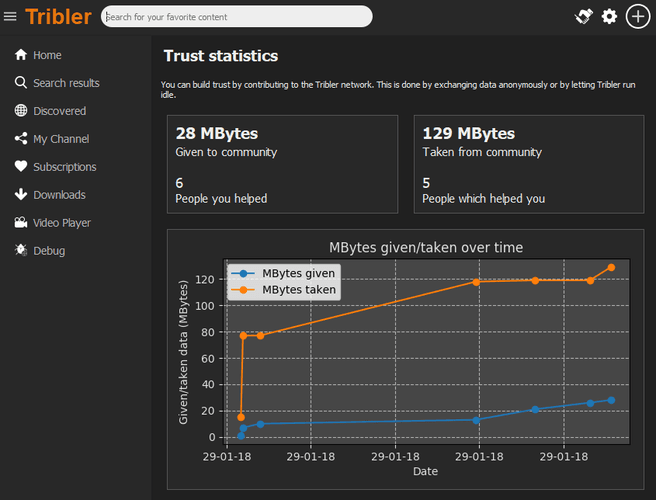
\includegraphics[width=1\linewidth]{related-work/tribler7.3.0.png}
        \caption{Tribler desktop interface, showing the bandwidth incentive system overview}
        \label{fig:tribler}
    \endminipage
\end{figure}

\section{DAO theory and technologies}
Important groundwork around the theory and implementation of a DAO has been done by \cite{jentzsch2016decentralized}. He notes that corporations originally work through people only, and this has two flaws: ``People do not always follow the rules, and they do not always agree what the rules require''. His paper illustrates a method that allows creating and maintaining organizations in which ``(1) participants maintain direct real-time control of contributed funds and (2) governance rules are formalized, automated and enforced using software''.

For an application to evolve without a company or a responsible group of people, decisions need to be made on protocol or feature additions and changes. We inspect the state-of-the-art of peer-to-peer technologies which enable autonomous communities to solve these problems by organizing themselves. In computer science, one approach to this is democratic voting based on voluntary proposals to change and improve the decentralized system. 

\cite{jentzsch2016decentralized} proposes a system based on the Ethereum blockchain, using smart contracts~\citep{buterin2014next}. In essence, any person that would like to join a DAO must be invited or pay a fee. All participants use tokens, to create proposals and to vote on proposals, so it uses a proof-of-stake mechanism. The paper also contains a solution for the majority owns minority attack: (an attacker with more than half of all tokens can make and accept a proposal to send all its tokens to itself) by allowing participants to split a DAO. 

One mobile implementation of this is a mini-app of the aforementioned TrustChain-Superapp (see fig. \ref{fig:trustchain-superapp-voter}). In this voting app, any participant of the organization can create a proposal for the community to vote on. Once a preset voting threshold is reached, the proposal is automatically accepted or denied. Bookkeeping of these proposals is done using the TrustChain distributed ledger technology~\citep{otte2017trustchain}. This voting app is an important basis for democratic decision making, but does not include code changes directly after proposals are accepted, so lacks app evolution. This protocol is based on proof-of-identity instead of proof-of-stake, as no tokens are involved.

\begin{figure}
    \centering
    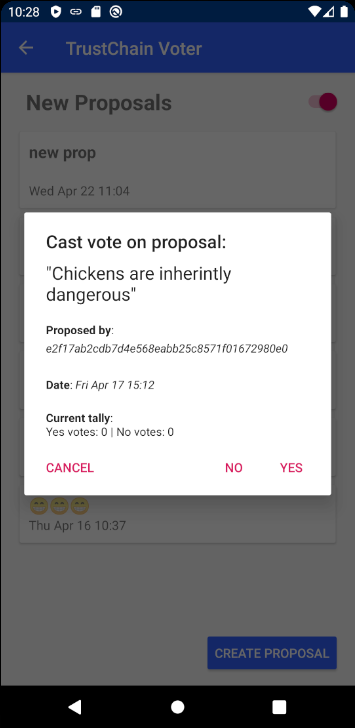
\includegraphics[width=0.3\linewidth]{related-work/trustchain-superapp-voter.png}
    \caption{Distributed democratic voting mini-app, showing proposals}
    \label{fig:trustchain-superapp-voter}
\end{figure}

\section{Decentralized content delivery networks}
\label{sec:decentralized-content-delivery}
A fully decentralized audio streaming service requires sharing and streaming audio files over a network of nodes in which any participant can start and run a node. Well-established examples of such networks are BitTorrent and IPFS.

\subsection{BitTorrent}
BitTorrent~\citep{bittorrentbep3} is an open peer-to-peer file sharing protocol. Any person can join the network and start sharing files, by making a torrent which contains the metadata of the files. Content is specified using SHA1 hashes of the files. Checksums are used to make sure no changes to the original torrent have been made upon receiving files. This way all files are immutably shared. BitTorrent has implementations for various systems, including Android. This means mobile devices can participate in uploading and downloading content, and can even build an autonomous phone-only file sharing system.

Torrent files contain a list of chunks (torrent pieces), which represent the different parts of the related file. Flawless streaming of media files over BitTorrent requires a smart algorithm to predict what file is requested next, and what torrent pieces should be loaded. BitTorrent originally relied on trackers to perform peer discovery, and trackers can become a central point of failure. However, since the introduction of the DHT protocol~\citep{bittorrentbep5dht}, finding peers in the network can be done by querying any known peer, which makes the network more decentralized. 

There are no differences between hosters and downloaders. Meaing, all participants have the same capabilities, so every user of the network can both download and upload content. A challenge of the BitTorrent protocol without extensions is incentivizing participants to host files. There are multiple solutions to this problem, discussed in \ref{sec:file-spreading-incentives}.

\subsection{IPFS}
The Inter-Planetary FileSystem, introduced by \cite{benet2014ipfs}, is a distributed peer-to-peer file sharing system in which any person can start a node and start uploading and downloading files. It uses a Distributed Hash Table to address content using a combination of SHA-256 hashes and hyperlinks. This means there is a global key-value store for all files (and file parts), in contrast to BitTorrent, which works with torrent swarms and trackers. IPFS uses an efficient graph implementation (a Merkle DAG) for addressing content and nodes. In addition, it removes duplications of files across the network. As IPFS uses a global key-value store for all files, every file hosting node needs to synchronize with the latest acyclic graph before it can start serving files.

End-users of content stored on IPFS can access content without supporting the network, so there is the possibility of free-riding. For example, users of the aforementioned Audius music streaming system are not required to run an IPFS node to improve the health of the network. In addition, there are no direct (financial) incentives to run an IPFS node, other than to help the network and to host content. 

\subsection{Comparison: IPFS and BitTorrent}
A notable difference between IPFS and BitTorrent is that IPFS makes a difference in file-hosting nodes and end-users (which only download files). BitTorrent does not make a distinction between these actors. In BitTorrent, every participant of the network has the capabilities to both upload and download content. Therefore a BitTorrent network using DHT is typically more decentralized than IPFS. 

IPFS uses a global file index using a hash tree, which means that every two file that produce the same hash are stored on the same index. This leads to de-duplication, which may result in better use of disk space, in comparison to BitTorrent.

% \begin{figure}
%     \minipage{0.45\textwidth}
%         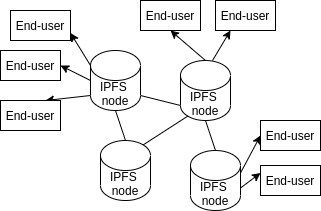
\includegraphics[width=1\linewidth]{related-work/decentralized-ipfs.png}
%         \caption{Decentralized file sharing structure: each node hosts nodes for some end-users}
%         \label{fig:decentralized}
%     \endminipage\hfill
%     \minipage{0.45\textwidth}
%         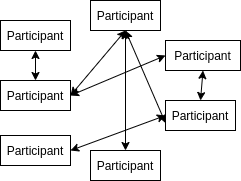
\includegraphics[width=1\linewidth]{related-work/distributed-bittorrent.png}
%         \caption{Distributed file sharing structure: each participant can exchange with each other participant}
%         \label{fig:distributed}
%     \endminipage
% \end{figure}

\section{Incentives for file hosting}
\label{sec:file-spreading-incentives}
In a DAO, the party responsible for hosting and spreading of files is not well-defined. To tackle the tragedy of the commons, entities should be incentivised just enough for the system to be sustainable and usable, but no more. An example incentive system is bandwidth tokens~\citep{de2018blockchain} as part of the Tribler system.

Tribler~\citep{pouwelse2008tribler} is a peer-to-peer system to share, download and stream multimedia. It has implementations for desktop environments and an Android prototype. It makes use of BitTorrent for file transfer and adds anonymization techniques on top of it. In addition, it makes use of its bandwidth tokens: an incentive system to increase cooperation between users, in order to achieve high availability of downloads. In essence, it subtracts tokens for downloading content from peers and rewards tokens for helping peers. An overview of the Tribler desktop interface can be seen in fig. \ref{fig:tribler}.

% FileCoin

% TODO READ/DISCUSS FOLLOWING RELATED WORK:
% https://github.com/javto/Tribler-streaming
% Decentralized Media Streaming on Android using Tribler

% STEEM
% PeerTube
\chapter{Design}
In this section we present the design of our software application MusicDAO. MusicDAO is a mobile music streaming and discovery app, with peer-to-peer payment to artists in the form of donations and subscriptions. The MusicDAO is fully decentralized by design. This means there are no intermediaries, third parties or proprietary servers needed. All users of the app form a community to share audio tracks and transfer money. Any user can join this community, publish their musical works and receive money from its listeners.

\section{A network without central control}
With the goal of distributing power in the music industry, every peer in the network will have the same rights and access to the same functions.

\section{Phone-to-phone connectivity}
Mobile phones have the largest share of any type of device using music streaming services. If the software that we design and implement runs well on a network consisting of only mobile devices, we can conclude that it will run well on better hardware (such as PCs) as well. For these reasons, we design our system to work on mobile phones only.

\section{Release model}
\label{sec:release-model}
A Release is an object describing a list of tracks that are published by a clearly identifiable artist or group of artists. For example, a Release can represent a single, and EP or an album. It is modeled as shown in fig. \ref{fig:release-model}. Release objects are shared between peers in the network. By discovering many of those objects, a user can see and browse through them to select a track to play. A Release object merely contains metadata of the tracks. We design the network to have a separate channel for downloading the track files. This is to enable fast discovery and
searching of Releases, as Release objects have a small byte size. 
\begin{figure}
    \minipage{0.2\textwidth}
        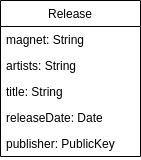
\includegraphics[width=\linewidth]{design/release-model.png}
        \caption{Release blocks structure as seen on TrustChain}
        \label{fig:release-model}
    \endminipage\hfill
    \minipage{0.3\textwidth}
        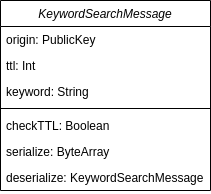
\includegraphics[width=\linewidth]{design/KeywordSearchMessage-model.png}
        \caption{KeywordSearchMessage object sent over IPv8 in MusicCommunity}
        \label{fig:keyword-search-message-model}
    \endminipage\hfill
    \minipage{0.5\textwidth}
    \endminipage
\end{figure}

\section{Identity and authenticity}
\label{sec:pki-design}
As we design a system that is fully decentralized, we cannot use a central database to record user identities. Therefore every user should generate a unique identity to be used in the network, and must be able to give proof of this identity. We use a public key infrastructure (PKI) which achieve these goals. Every user stores their private and public key on their device, and only share their public key. The keypair has a mathematical property that allows verification of messages that are signed with a private key. By comparing the public key of a peer with their signed message, anyone can verify the authenticity of the message.

In the context of MusicDAO we use this PKI to proof ownership of Release objects. All Release objects are signed using the owner's private key and the signature is added to the object. Any user receiving this object can verify its authenticity.

\section{Distributed storage}
Central to our system is sharing downloading and storage of audio files and Release objects (see \ref{sec:release-model}). To design a system which has no middlemen or regulators for publishing Releases, and has no central control, a distributed storage system is required. This storage system should have the following properties: immutability (data cannot be tampered with), resiliency (data should be available as long as users want it) and rigorous duplication (all objects should live on multiple devices so they do not disappear when requested). Distributed ledger technology (DLT) allows for these properties, so we design our system with a DLT as a major component.

\section{Distributed downloading and uploading}
To be able to have low latency for discovering and playing music tracks, while using no central nor high-throughput servers, the network demands participants to upload content continuously. We design the app to, by default, use the network capabilities of the mobile device to upload content as much as possible. This is constrained by networking hardware, data subscription plans and other software running on the phone.

\section{Distributed search algorithm}
For searching content we use a simple distributed algorithm called XYZ (cite). Pseudocode of this algorithm is shown in fig. X. It asks peers around for content tagged with some keyword. When a peer finds a match on their local database, it sends this Release object to the original asking peer. Otherwise it forwards the query to their neighbours, after reducing the time-to-live property by 1. The messages stop being forwarded once their time-to-live property hits below 1. The structure of search messages are shown in fig. \ref{fig:keyword-search-message-model}.

\section{Direct payments without intermediaries}
As we are designing a system with no intermediaries, it should be possible to give money directly to artists. Cryptocurrency allows for peer-to-peer payments which achieve this goal, so we use this in the MusicDAO. Cryptocurrency payments will be used for two different functionalities: a user can send a donation to an artist, or a user can pay artists using a monthly subscription system. This subscription system pays artists that the user listened to, using the Artist Income Division Algorithm (see \ref{sec:aida-design}).

\subsection{Wallet}
Cryptocurrency implementations allow for private/public key-pairs which can be interpreted as a kind of wallet; the funds can only be unlocked by a holder of the private key. In the case of MusicDAO we design the app to include a wallet for every user. To receive money, every artist should share their public key to all of their listeners. To achieve this, the public key of their cryptocurrency wallet is included as a property of the Release objects (see \ref{sec:release-model}). As there are no institutions or banks involved in storing money, users will be required to keep their private key safe.

\subsection{Artist Income Division Algorithm}
\label{sec:aida-design}
To provide a stable income for artists, in the form of reoccurring payments, we design the Artist Income Division Algorithm. This algorithm calculates how periodic subscription money is split into payments to artists. The user can enable a periodic payment. This money is then divided over the artists the user listens to, in proportion to the amount of interaction with each artist. Interaction can be measured in e.g. time listened, plays or feedback in the form of likes. The details of this division is explained in the implementation section of AIDA (see X).
\todo[inline]{This sec may be removed}
\chapter{Implementation}
The application is implemented as a `mini-app' of the \textit{TrustChain Superapp}~\citep{mattskala2020}. This follows the concept of super apps~\citep{kpmg2019superapps}. The app is published on the Android Play Store\footnote{\url{https://play.google.com/store/apps/details?id=nl.tudelft.trustchain}} and its code is publicly available\footnote{\url{https://github.com/Tim-W/trustchain-superapp}}. As programming language Kotlin is selected, as it is the preferred language for Android development~\citep{googleio2019}. Moreover the underlying technology stack is also written in Kotlin, so this allows for neat integration. This section describes the implementation choices, usage of external libraries and presents the user interface of MusicDAO.

\section{Identity and authenticity}
We implement the public key infrastructure as described in \ref{sec:pki-design}. We use the identity system proposed by \cite{mattskala2020}. All Release blocks (as with all blocks) created on the TrustChain are assigned an identity of the creator. This is a public key using \textit{Curve25519} elliptic-curve cryptography. Every device running the MusicDAO will receive a public/private key-pair upon first launch. While the public key ultimately shows the identification of the device, it can also be used as identification of the artist owning the device. Currently there is no multi-signature support implemented. This means that in the case of a group publishing a Release, there is only one public key representing the whole group. Every artist, and every unique collaboration between artists should generate their own key-pair to describe ownership of the Release.

\section{Metadata storage and discovery}
\subsection{Release blocks}
Releases are objects that represent an audio release produced by one or more artists. This can be an album, an EP, a single, or a podcast. Release objects are stored on the TrustChain, and are exchanged between peers that are part of the MusicCommunity (see \ref{sec:searching-musiccommunity-impl}). These objects are structured as shown in \ref{fig:release-model}. The \textit{magnet} property contains a magnet link which holds all additional information about the contents of the Release, such as the torrent file list, size and tracker URLs. The \textit{publisher} property contains the public key of a Bitcoin wallet which is owned by the creator of the Release. This public key is an identity of the owner of the record (either the artist, band or label). This allows only the owner to receive funds sent by listeners, and no other middlemen (apart from miners).
% When a torrent is created from a local file list, the TorrentInfoName value is established. 

\subsection{MusicCommunity and keyword search}
\label{sec:searching-musiccommunity-impl}
The MusicCommunity extends the TrustChainCommunity with additional methods \textit{performRemoteKeywordSearch} and \textit{onKeywordSearch}. These methods enable searching for content using a keyword, both locally and remotely. These methods test each \textit{title}, \textit{artists} and \textit{date} field of each Release block against a \verb|contain(keyword)| filter. This means: if the keyword is contained in one of those values, it is added to the results.

When the user performs a search, the local database is filtered first to find matches. If there are less than \(x\) results, the device sends a KeywordSearchMessage (see X) to a maximum of \(P\) known peers in the MusicCommunity. This asks neighbours to inspect their local database to find matches for the same query. Upon receival, the peer subtracts 1 from the time to live (TTL) field. If the peer finds a match, it sends the corresponding TrustChain block directly back to the original asker, appointed by the \textit{origin} field. This contains the IPv8 \textit{peer ID}~\citep{mattskala2020} of the peer that initiated the search. Otherwise, if the time to live (TTL) is more than 1, the peer forwards this KeywordSearchMessage (see \ref{fig:keyword-search-message-model}) to other peers. Our keyword search is implemented with default values of \(T=1, P=20, x=5\) (where \(T\) is the TTL).

\section{Networking}
We implement audio track uploading, downloading and streaming using BitTorrent. This technology has shown to run well on mobile devices (cite), allows for extensive configuration and flexible uploading (seeding) strategies. Moreover it supports transfer over local area network and discovering peers in a distributed hash table. It is a well-established technology, as it was released in 2001.

We use the JLibtorrent\footnote{\url{https://github.com/frostwire/frostwire-jlibtorrent}} implementation by Frostwire, which is a Java swig interface for libtorrent\footnote{\url{https://www.libtorrent.org/}}.
\subsection{Torrent creation and sharing}
\label{sec:torrent-creation}
In our application, a user can select local audio tracks, after which a torrent file is generated with the corresponding metadata. Alternatively, the user can paste a preexisting torrent magnet link to use for the Release block, as shown in \ref{fig:select-tracks}. The creation of torrents by the app happens as follows. First, the user presses the \textit{Select Local Audio} button in the release creation dialog (see \ref{fig:submit-release-dialog}). Afterwards, the user selects one or more tracks to add (see \ref{fig:select-tracks}). In the background this creates a torrent file, which is stored on the mobile device and added to the ContentSeeder (see \ref{sec:content-seeding}). Finally, by using the computed infohash and file list, the magnet link of the torrent file is created and added to the \textit{magnet} field of the Release block.

By default, the torrents created using MusicDAO are marked as `trackerless' meaning that torrent peers are found using a distributed hash table~\citep{dht2019} (specifically, mainline DHT\footnote{\url{https://www.libtorrent.org/dht_extensions.html}})instead of centralized trackers. This is to keep the app independent on connectivity on trackers and pushes towards a fully distributed system.

In addition, the app enables the local peer discovery (LPD)~\citep{bittorrentbep142015} functionality of BitTorrent. This allows for finding peers and transmitting torrent pieces over local area network. This results in higher transmission speed and lower latency for content that is stored in the cache of devices nearby. For example, if device A is looking for track X, and device B has this track cached and is active on the same local area network, this track can be found and buffered quickly from A.
\begin{figure}
    \minipage{0.3\textwidth}
        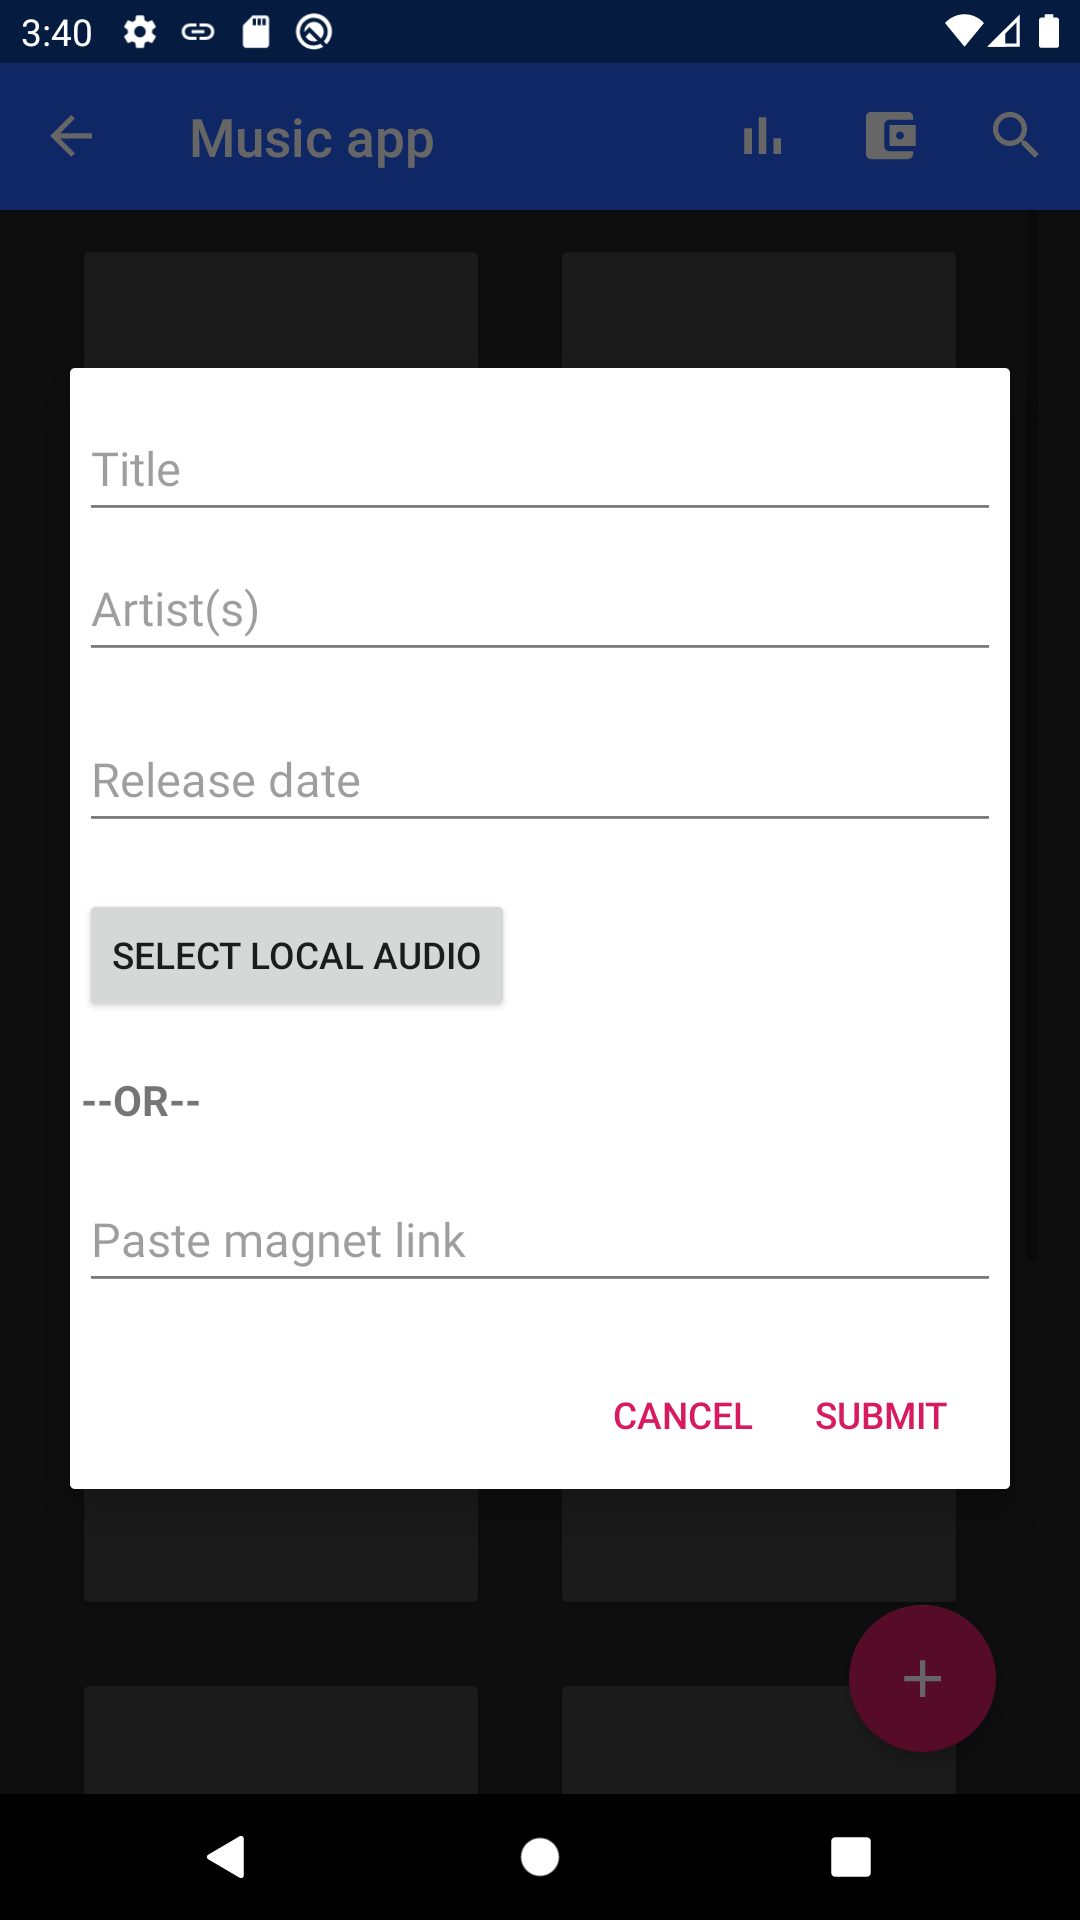
\includegraphics[width=\linewidth]{implementation/screenshot-select-tracks.png}
        \caption{Dialog for creating and publishing a new Release}
        \label{fig:submit-release-dialog}
    \endminipage\hfill
    \minipage{0.3\textwidth}
        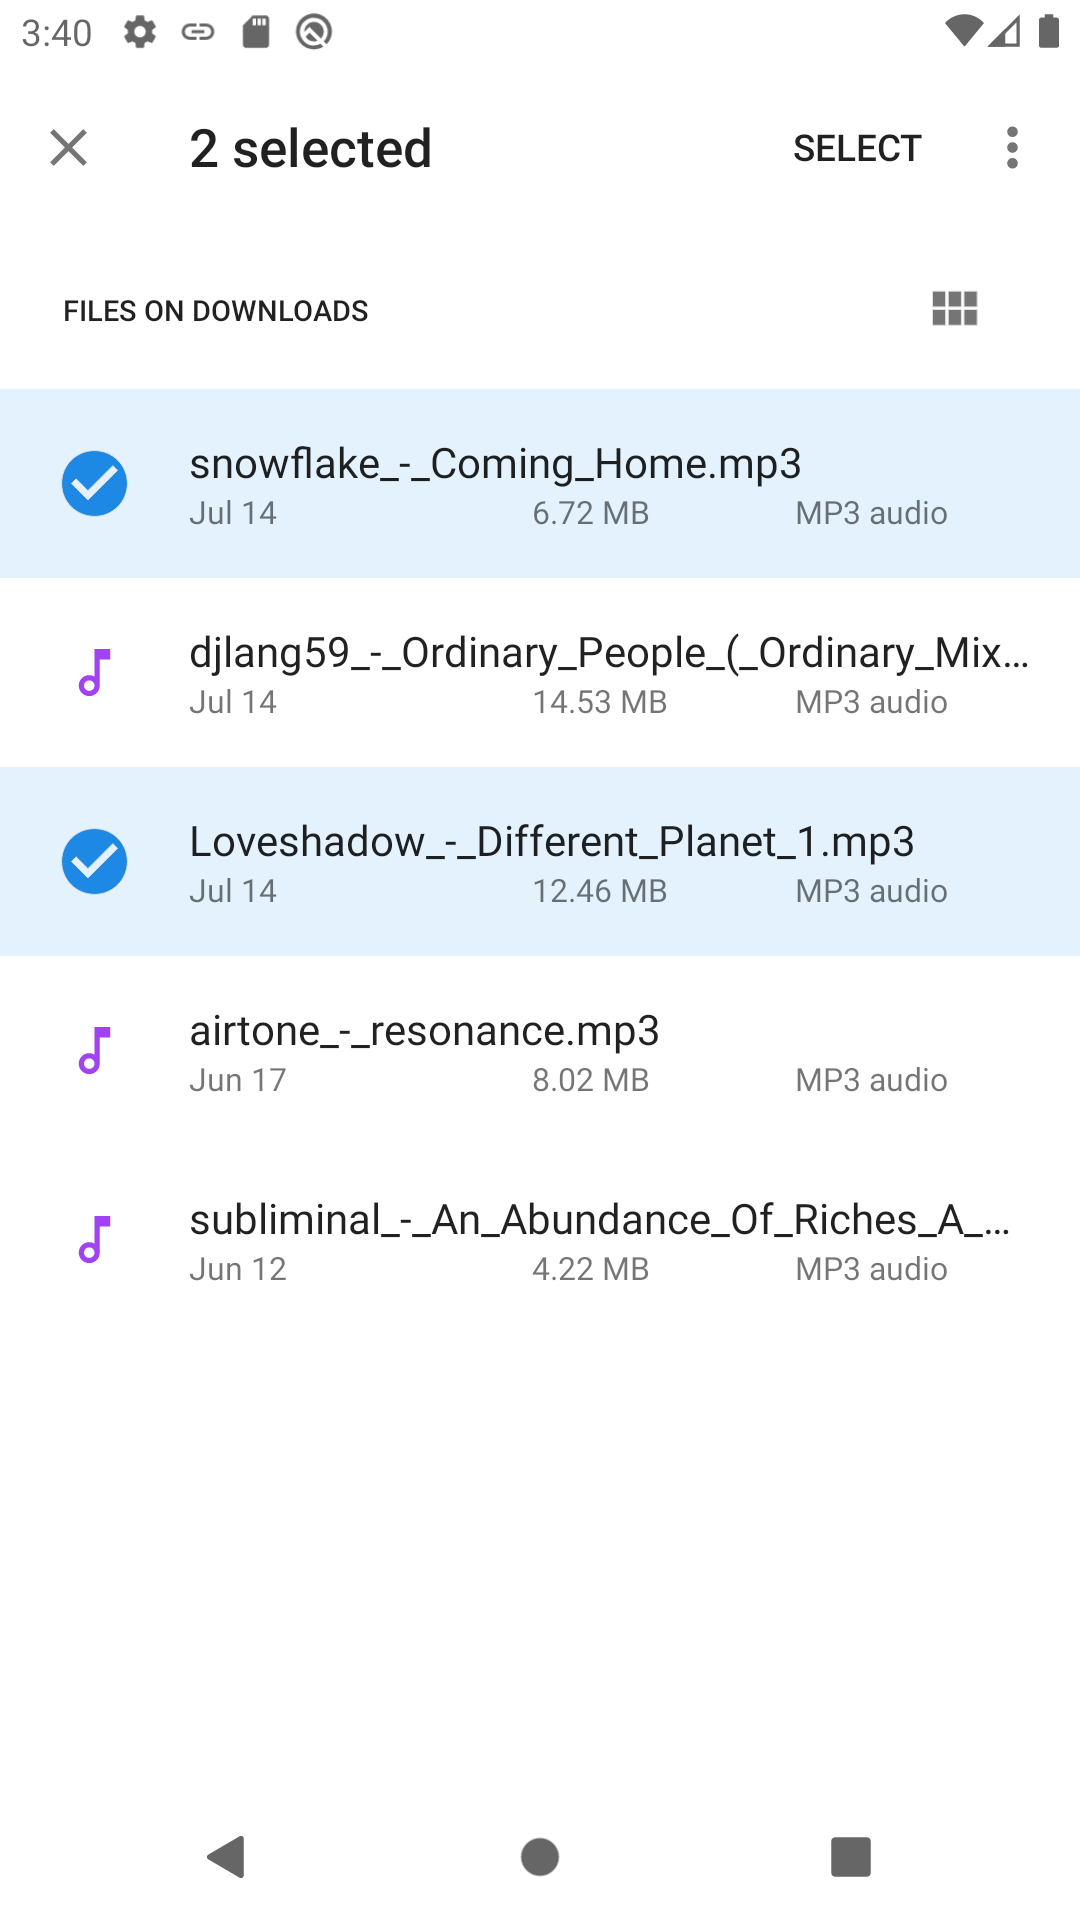
\includegraphics[width=\linewidth]{implementation/screenshot-submit-release.png}
        \caption{Selecting local tracks for creating a new Release}
        \label{fig:select-tracks}
    \endminipage\hfill
    \minipage{0.3\textwidth}
    \endminipage
\end{figure}
\subsection{Content seeding}
\label{sec:content-seeding}
Seeding of content is implemented using a simple continuous mechanism. On startup, the ContentSeeder class (see X) spawns a background thread which iteratively scans all torrent files in the local cache directory of the app. There is an upper threshold for how many torrents are selected for seeding. This threshold \(T\) is currently set to \(T=10\). The ContentSeeder uses a last-in-first-out heuristic: the top \(T\) most recent created/received torrent files are seeded.
\section{Caching}
The app implements both caching of tracks and metadata, to enable fast browsing and playback of tracks. As described in \ref{sec:torrent-creation}, only magnet links are shared on the TrustChain blocks. When the user opens a playlist for the first time, torrent metadata is fetched from peers for the corresponding magnet link. Once this metadata is received, it is written to a new .torrent file in the \textit{cache directory}\footnote{\url{https://developer.android.com/training/data-storage}} of the app. This can then be picked up by the ContentSeeder (see \ref{sec:content-seeding}). The tracks are also stored in the cache directory, in subdirectories identified by the \textit{name}~\citep{bittorrentbep3} property of the torrent metadata. The process of browsing playlists, loading metadata and selecting tracks using caching is shown in fig. \ref{fig:playing-tracks}.
\begin{figure}
    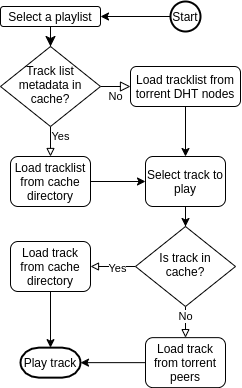
\includegraphics[width=0.3\textwidth]{implementation/playing_track.png}
    \caption{Browsing and playing tracks}
    \label{fig:playing-tracks}
\end{figure}

\section{Music Player and Streaming}
Playing music is implemented using ExoPlayer 2.10\footnote{\url{https://github.com/google/ExoPlayer}}. This music player library is suitable as it allows for playing tracks that are partially loaded, which enables streaming.
\subsection{Priority handling}
To provide the user with selected content as soon as possible, we implemented a system which sets priorities on certain tracks and torrent chunks. This uses the piece priorities system in libtorrent, which range from the integers 1 (normal) to 7 (highest) (see libtorrent Manual\footnote{\url{https://www.libtorrent.org/manual-ref.html\#file-format}}). When a user selects a track, this track is given a \textit{file\_priority} of 5. This is a higher priority than that of other files, so JLibtorrent asks actively for peers who have this file. In addition, the first 5  pieces of the selected track are given a \textit{piece\_priority} of 7, so that the first seconds of the track are buffered quickly and the user can start streaming early.
\subsection{Seeking and buffering}
The music player tries to play the track once a satisfactory portion is loaded. This is implemented as follows. Upon seeking a part of the track, the torrent piece index on which the cursor is located is calculated. Afterwards, the piece at this index and the 5 consequent pieces are given a \textbf{piece\_priority} of 7, which is higher than the other pieces. Once at least 2000 ms from the cursor is buffered, the music player starts playing the track. This way the user can start playing the portion of the track they are most interested in quickly.
\section{Donations and payments}
\subsection{Bitcoin RegTest network}
We created a public Bitcoin RegTest environment\footnote{\url{https://developer.bitcoin.org/examples/testing.html\#regtest-mode}} to test peer-to-peer Bitcoin donations and payments. This creates a new `clean slate' Bitcoin blockchain and allows for full control over the chain and miners. This enables a test environment that is useful for experiments, as we can tweak the block generation speed and keep track of all transactions registered on the closed-off blockchain.
\label{sec:regtest-network-impl}
\section{Interface}
\subsection{Playlist overview}
The playlist overview screen, as shown in \ref{fig:screenshot-home} is the screen that is first shown upon starting the MusicDAO. Here the user is presented a list of playlists, loaded from their local TrustChain database. Currently, each Playlist fragment corresponds to exactly one Release block (see ref). In the background runs an iterative process which checks whether new playlist content is found, and re-renders the view if necessary. The playlists are sorted on their torrent swarm health in ascending order. 
\begin{figure}
    \minipage{0.3\textwidth}
        \includegraphics[width=1\linewidth]{implementation/screenshot-superapp.png}
        \caption{The app is integrated as a mini-app in the IPv8 Superapp catalog}
        \label{fig:screenshot-superapp}
    \endminipage\hfill
    \minipage{0.3\textwidth}
        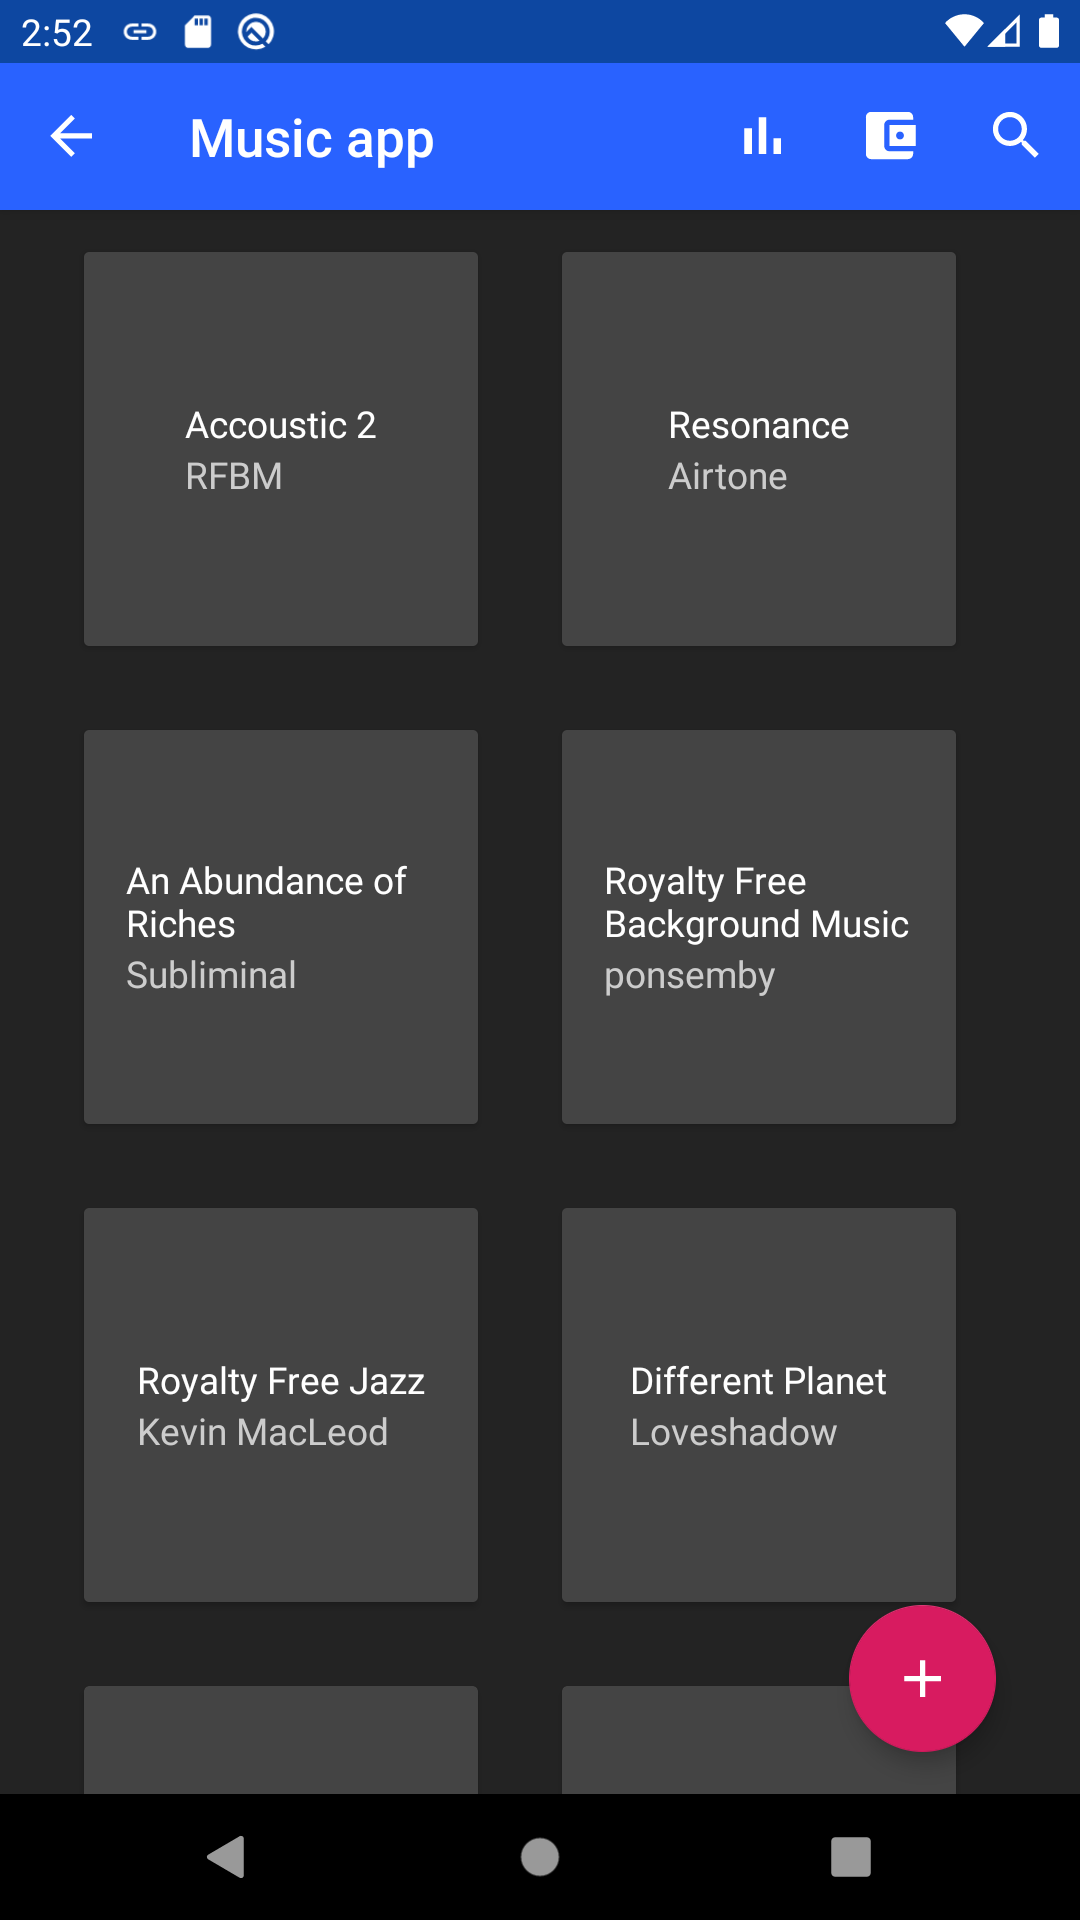
\includegraphics[width=1\linewidth]{implementation/screenshot-home.png}
        \caption{The playlist overview screen, which is the entrance screen}
        \label{fig:screenshot-home}
    \endminipage\hfill
    \minipage{0.3\textwidth}
        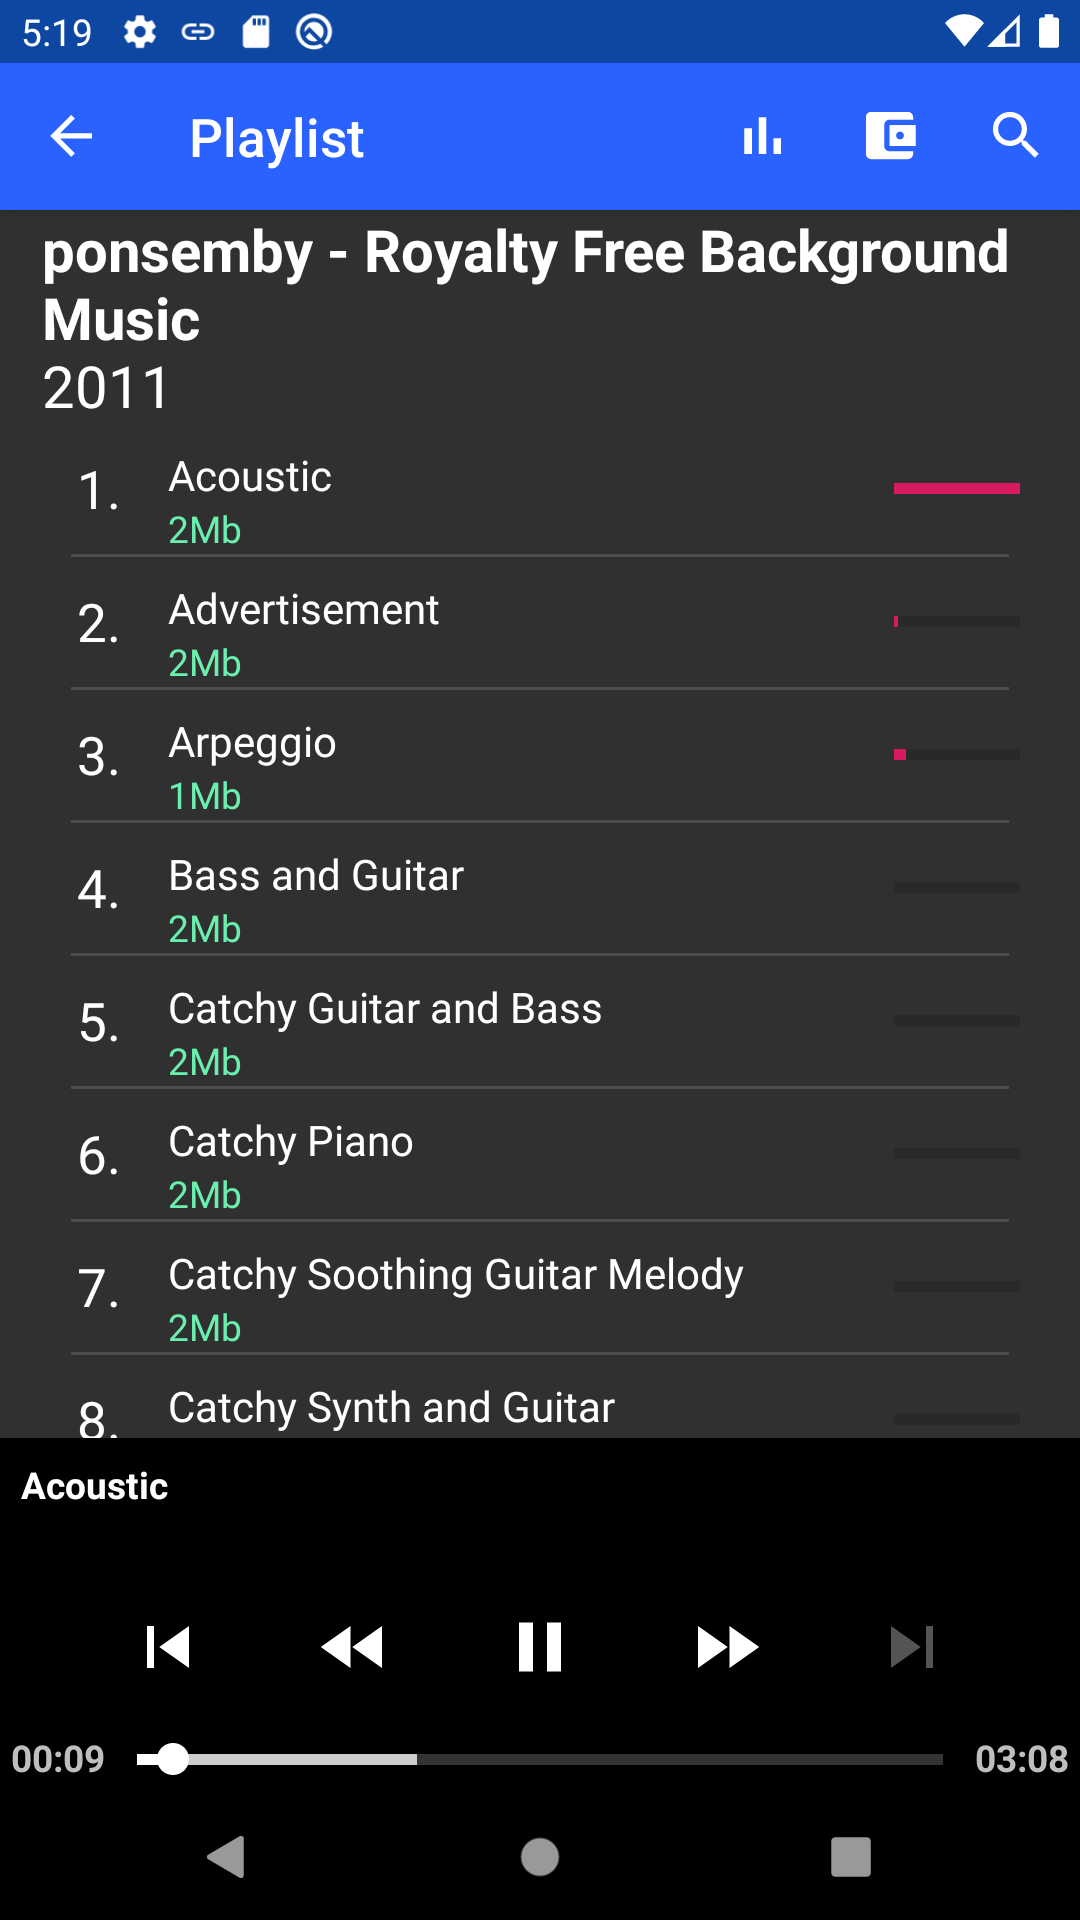
\includegraphics[width=1\linewidth]{implementation/screenshot-playlist.png}
        \caption{Playlist fragment, showing all tracks of one Release}
        \label{fig:screenshot-playlist}
    \endminipage\hfill
\end{figure}
\subsection{Playlist fragment}
A Playlist fragment displays one Release object. The playlist fragment shows its list of tracks and other metadata, such as the title and artists of the Release (see \ref{fig:screenshot-playlist}). For each track the file size is displayed, and a loading indicator on the right side. This shows, in real time, how much of the track is downloaded. In the example of \ref{fig:screenshot-playlist}, the first track is fully loaded.
\subsection{Wallet}
Each device participating in the MusicCommunity is given a private/public wallet identity upon installation of the MusicDAO. The wallet interface (fig. \ref{fig:wallet-sync}) shows synchronization status of the RegTest network (see \ref{sec:regtest-network-impl}). Once the wallet is fully synchronized with the blockchain, the private key and balance are displayed as shown in fig. \ref{fig:wallet-balance}. 

Upon browsing a playlist, if the \textit{publisher} field is present in the corresponding Release object, a donation button is displayed as shown in fig. \ref{fig:tip-artist}. When pressing this button, the user can select an amount and make a direct donation to the artist or band, in the form of a bitcoin transaction from their wallet. The user enters a value in USD and the corresponding amount in bitcoin is calculated and shown when this field is edited. This is implemented using the XChange library\footnote{\url{https://github.com/knowm/XChange/releases/tag/xchange-5.0.1}} connecting to the Binance trading platform\footnote{\url{https://www.binance.com/en/trade/BTC_USDT}}. After confirmation, the transaction is registered on the RegTest network (see \ref{sec:regtest-network-impl}). 
\begin{figure}
    \minipage{0.3\textwidth}
        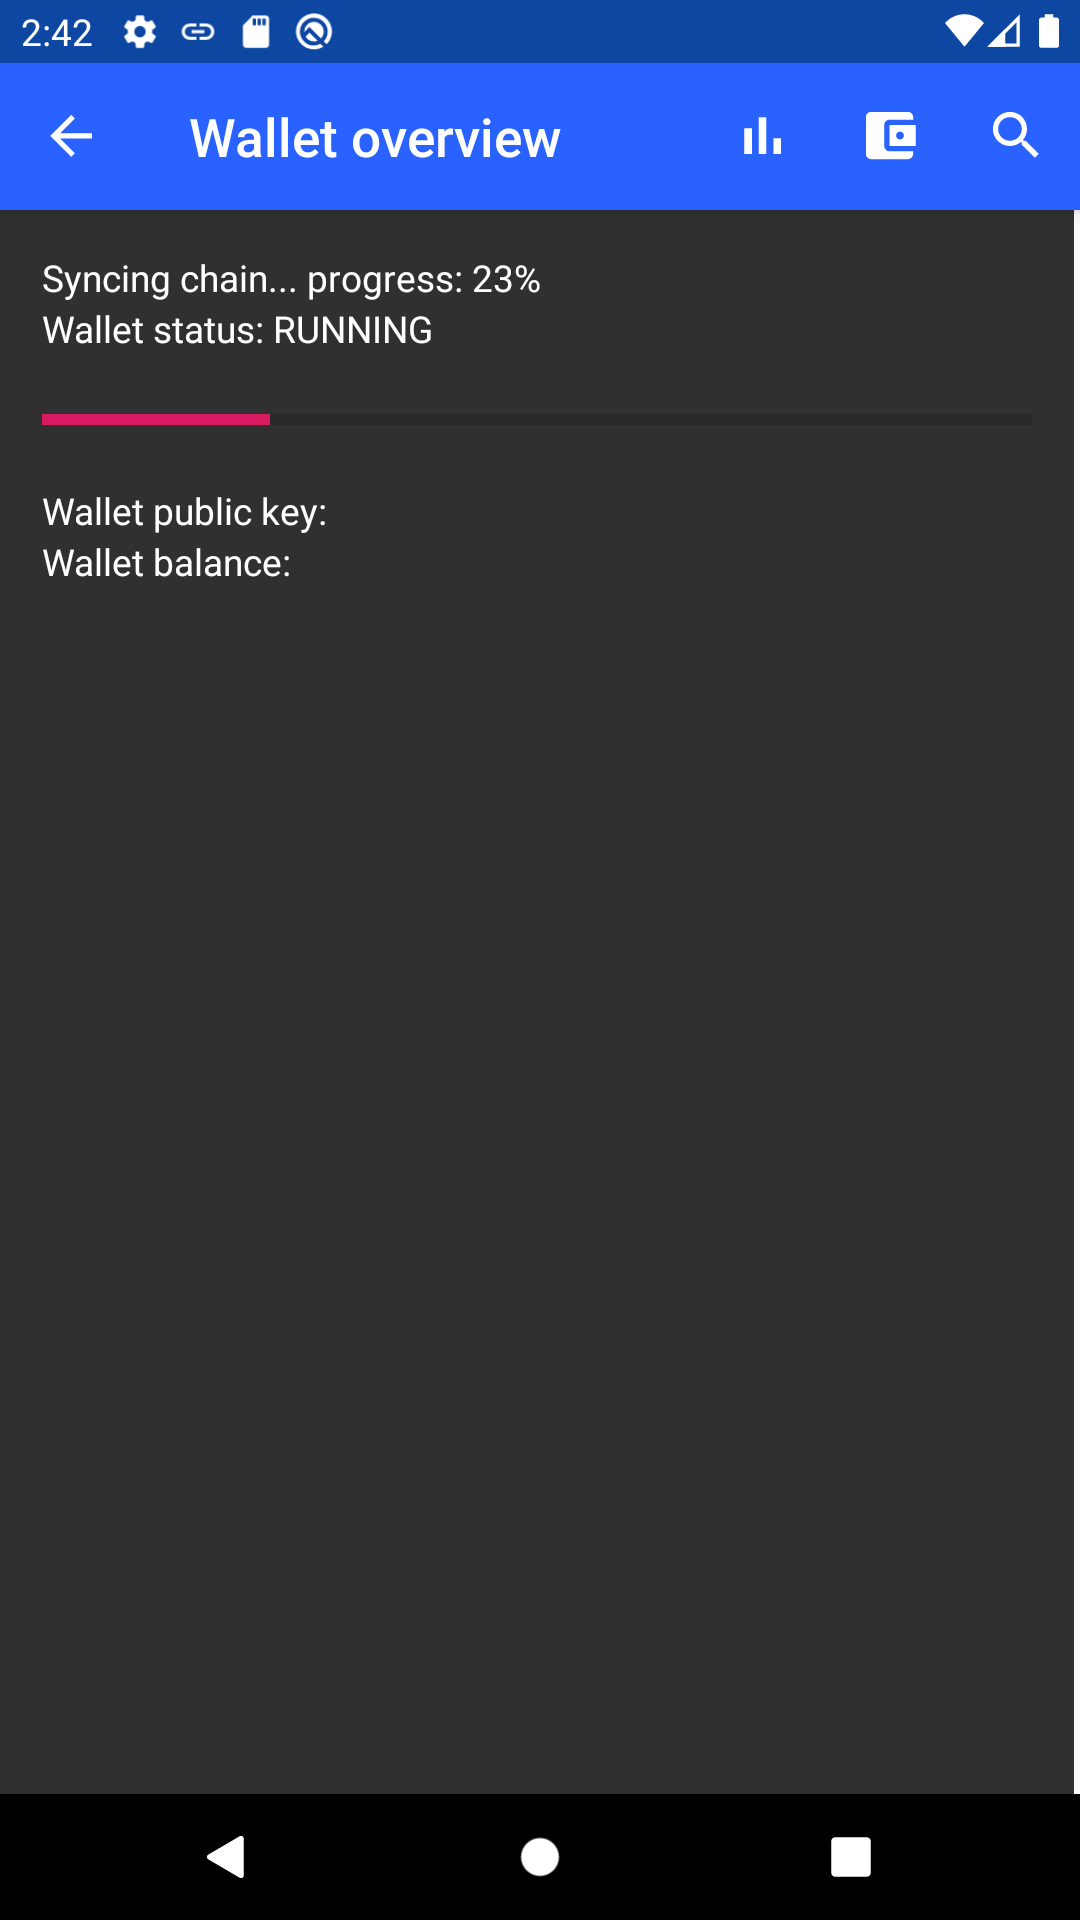
\includegraphics[width=1\linewidth]{implementation/wallet-sync.png}
        \caption{Synchronizing with the Bitcoin RegTest environment blockchain}
        \label{fig:wallet-sync}
    \endminipage\hfill
    \minipage{0.3\textwidth}
        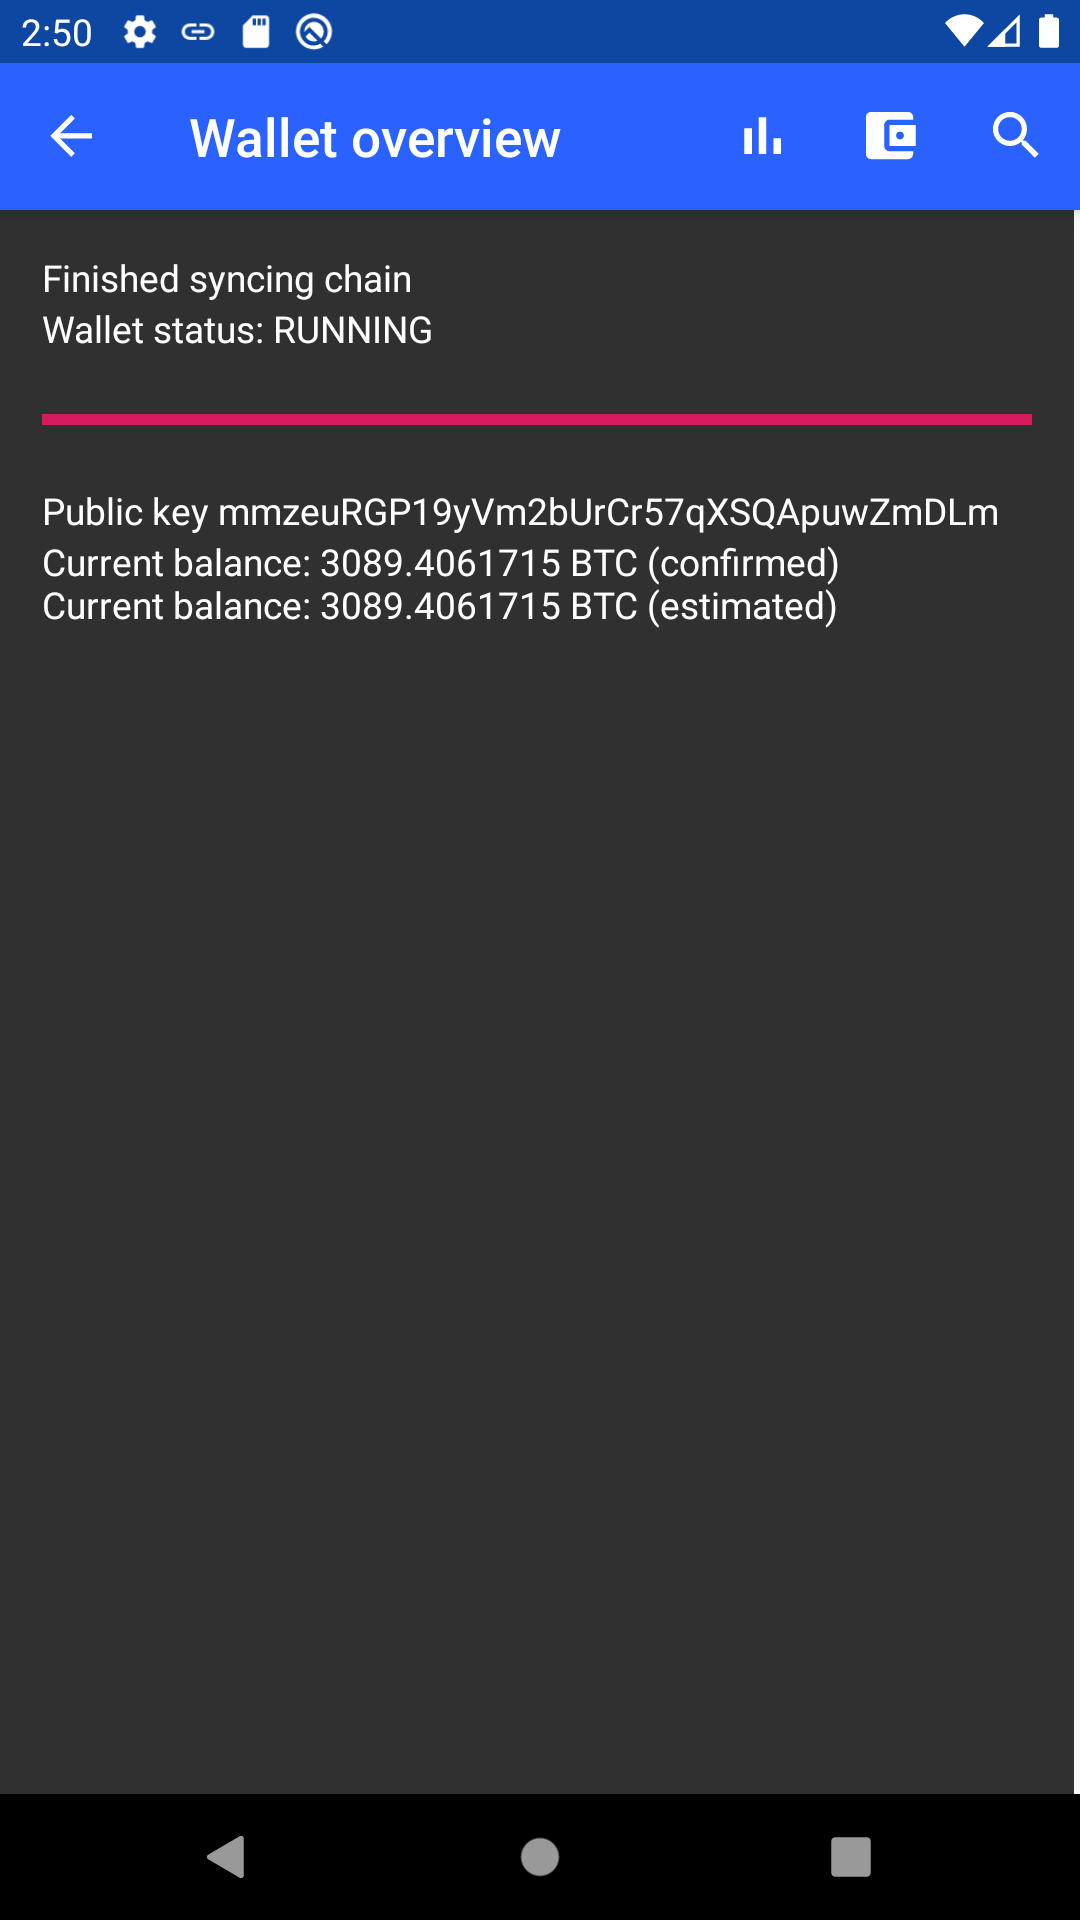
\includegraphics[width=1\linewidth]{implementation/wallet-balance.png}
        \caption{Wallet overview and balance after synchronizing}
        \label{fig:wallet-balance}
    \endminipage\hfill
    \minipage{0.3\textwidth}
        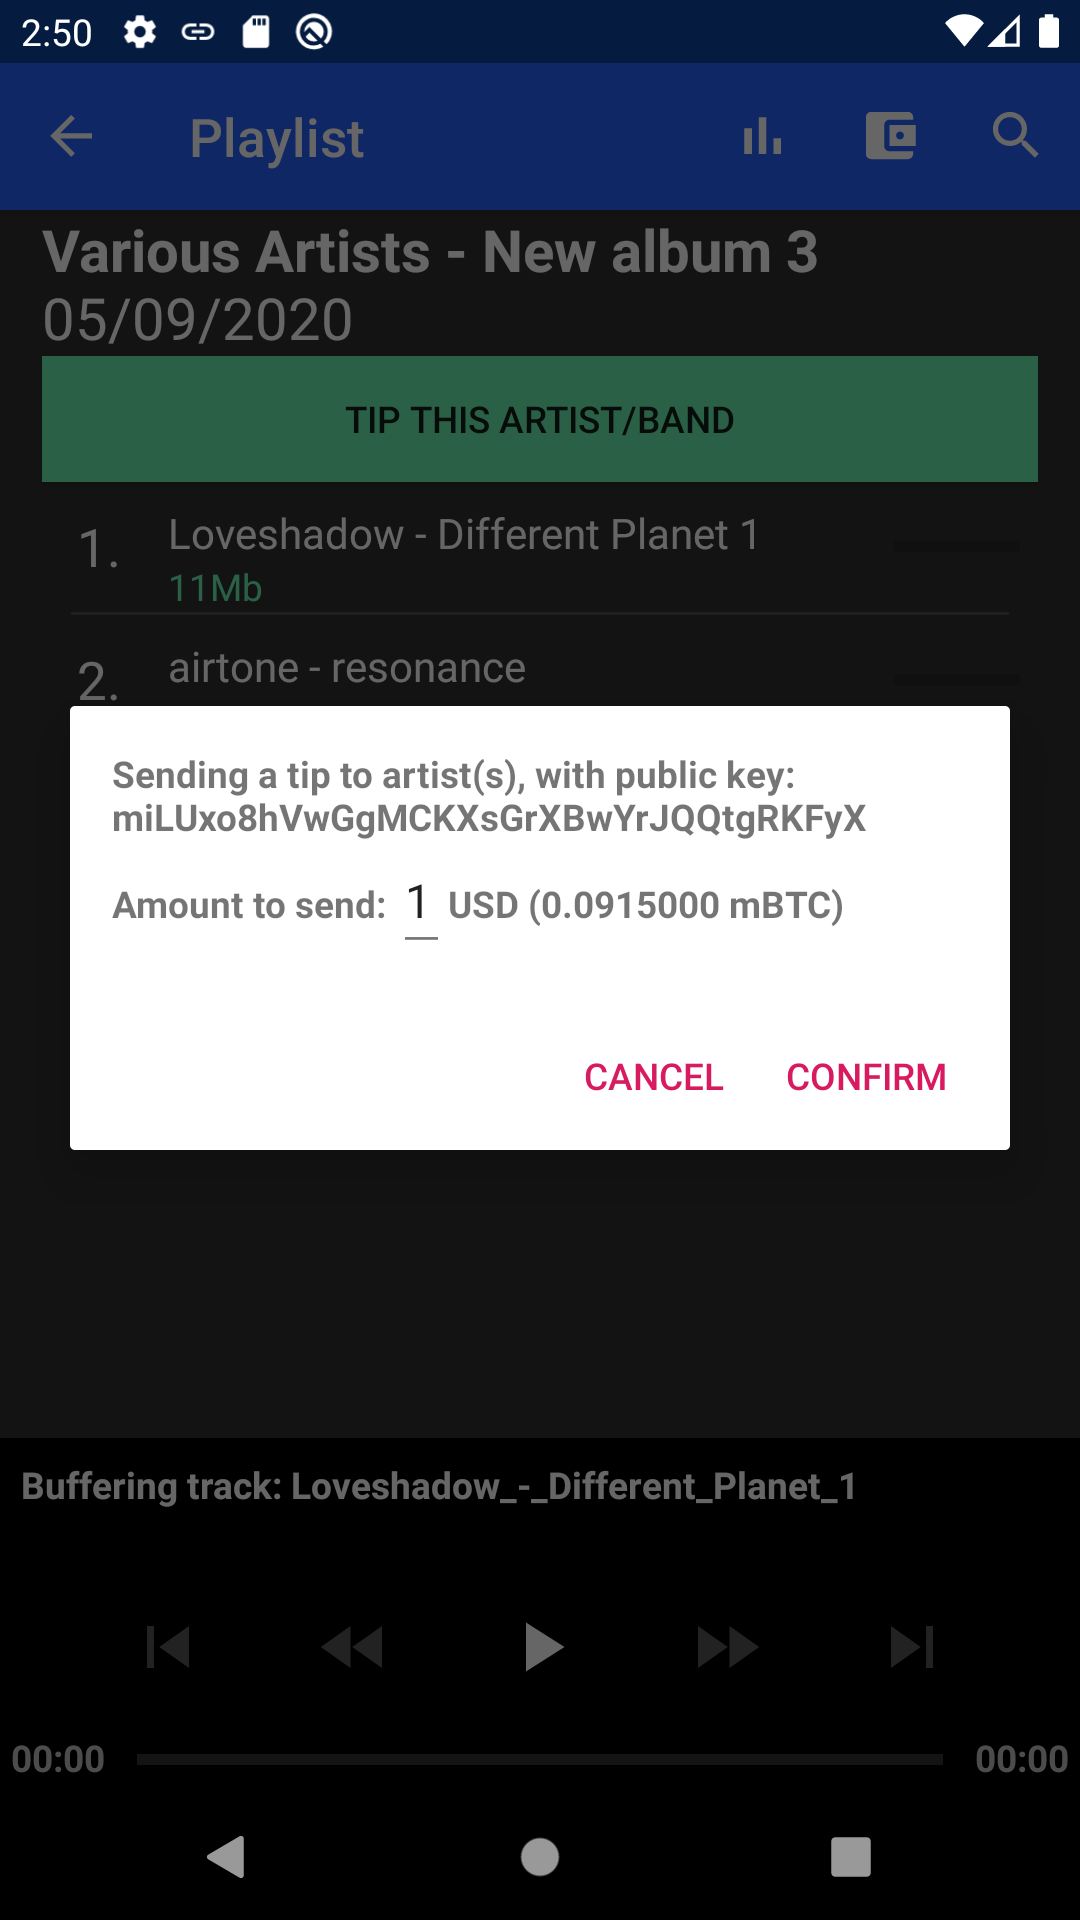
\includegraphics[width=1\linewidth]{implementation/tip-artist.png}
        \caption{Sending a tip to an artist or band}
        \label{fig:tip-artist}
    \endminipage\hfill
\end{figure}
\chapter{Conclusion and Future Work}
This thesis presents a novel framework for building a robot economy in software. This framework allows for designing and implementing software for the common good: software that (1) handles financial transactions in a fair way (2) as decided by democratic engagement, (3) runs transparently and autonomously, (4) is open to any participant (permissionless), (5) is decentralized and leaderless, (6) supports a self-evolving codebase, and finally (7) can make intelligent decisions on its own using AI.

This thesis presents a music streaming alternative for the Big Tech industry: we implemented our framework in order to build a fully working decentralized music streaming, publishing and discovery mobile app with peer-to-peer donations. In this proof-of-concept called MusicDAO, we applied the theory of the robot economy in software to an industry of which the core contributors (artists) suffer majorly from centralization on the Internet: the music industry. Most music streaming platforms take a 20-40\% cut of music revenue; MusicDAO takes 0\%. MusicDAO implements 1, 3, 4 and 5 of the key features of a robot economy in software (see above).

MusicDAO is completely free of label and platform intermediaries taking large revenue cuts. It forwards $>99.99\%$ of all music revenue to artists. All money flow is public and transparent. Artists using our DAO can be independent and self-publishing. Apart from the \textit{music platform oligarchy}, it also surpasses the \textit{label oligarchy} as it requires no music label to publish music.

MusicDAO implements a peer-to-peer audio streaming algorithm, which is able to stream any BitTorrent audio swarm. Its buffer loading time does not reach industry standards yet but this can be improved by more optimized pre-fetching and piece ordering algorithms. 

Our system is not yet resilient against free-riding, spam attacks or sybil attacks. Preventing such attacks is an active developing area in distributed systems research.

\section{Generality: beyond music}
The framework presented in this thesis can be applied to many other domains beyond music. Most functions of corporation-run centralized platforms are already automated, and handled by AI or robots. It can transform Internet platforms, or even complete value chains that currently have unfair or opaque money flows. One may think of a production and sales chain with no retail cut, or a video publishing network with a subscription model without intermediaries. This thesis aims to be a step into an evolving research direction, \textit{infrastructure for the common good}: autonomous software that works in favor of its user community instead of companies or profit.

\section{Future research directions}
In the MusicDAO proof-of-concept, there is no use of intelligent robots. Decision making based on AI is the next key step to the robot economy in software. We envision a symbiotic interaction between humans and robots: humans vote for the baselines and rules within which robots play, while robots use AI such as machine learning or evolutionary algorithms to perform tasks and make decisions. 

Content moderation is a key ingredient of any Internet platform. In MusicDAO, any music that is published is automatically admitted to the network. Therefore the network does not automatically remove any duplicates (copies), illegal remixes or other illegal audio. Using DAO and intelligent robots, a system can be created in which robots moderate content using AI, while humans democratically vote on the rules for content.

Ongoing research into Self-Sovereign Identity (SSI) can fix part of this problem: SSI can create a certain passport for content creators, with which creators can prove their identity and thus ownership of certain content.

%\section{Future research directions}
%\begin{itemize}
%    \item Actual AI used for decision making
%    \item Content moderation by voting and/or AI
%    \item Continuous, democratic code evolution (based on voting protocol), %bountysource.com, secure plugin system related work
%    \item Artist identity/passport, relate to Self-Sovereign Identity %related work (SSI)
%    \item Towards fully fair, transparent and open democratic systems for %the common good (discuss what the holy grail is of a Robot Economy)
% Active democratic engagement: forums, voting rounds (procedures), public interaction/discussion, etc.
%\end{itemize}

Streaming income is only a part of revenue from music. MusicDAO can be extended to include other revenue flows to artists, to make also those incomes higher and more transparent for artists. Possibilities are e.g. live concert tickets, merchanidise or physical audio sales.

A robot economy is highly susceptible for the problem of \textit{determining responsibility} when things go wrong. For example, a software bug may occur or a robot can make an unexpected monetary transaction. This challenge requires research into new theories and ideas in the context of law and philosophy for the robot economy.

% In the current software implementation, when a user makes a donation, this transaction is atomic and can only go to one wallet. An automatic splitting system between different artists of one group or band has not been implemented yet.

%% Use letters for the chapter numbers of the appendices.
\appendix

%\input{appendix-a}
\bibliographystyle{apacite}
\bibliography{report}

\end{document}

